\documentclass[12pt, a4paper]{article}
\usepackage{triada}
\usepackage{subfigure}
\usepackage{float}
%\usepackage{enumerate}


\graphicspath{{eps/}{png/}}
\begin{document}

\tableofcontents

\newpage

\section{Задание 1}
\subsection{Постановка}
\begin{enumerate}
\item На основе генератора схемы Бернулли построить датчик для биномиального и отрицательного биномиального 
распределений.
\item На выборке объема $5000$ проверить эмпирически закон больших чисел.
\item Произвести $N=1000$ испытаний бернулли с вероятностью $\frac 12$ и интерполировать траекторию процесса $Y(t_n)=\frac{S_n}{\sqrt{N}}$ ломаной на отрезке $\left[0,1\right]$. $t_n = n/N,\ \linebreak S_n = \sum\limits_1^n X_n,\ X_n\in\left\{-1,1\right\}$
\end{enumerate}
\subsection{Теоретическая часть}
\subsubsection{Определения и свойства}
\begin{df}
Случайная величина $X$ имеет \textit{распределение Бернулли} с параметром $p$, если она принимает лишь два значения, обычно $0$ и $1$, причем \[ \P(X = 1) = p,\ \P(X = 0) = 1-p. \]
\end{df}
\begin{df}
\textit{Схема Бернулли} состоит в проведении $N$ экспериментов (\textit{испытаний}), результатом каждого из которых может быть удача с вероятностью $p$ либо неудача с вероятностью $q=1-p$.
\end{df}
\begin{df}
\textit{Биномиальное распределение} $\Bi(n,p)$ --- распределение числа успехов в схеме Бернулли с $n$ экспериментами и вероятностью успеха $p$. 
\end{df}
Случайная величина $Y = \sum\limits_1^n X_i$, где $X_i$ имеют распределение бернулли с параметром $p$, имеет распределение $\Bi(n,p)$.
\begin{df}
\textit{Отрицательное биномиальное распределение} $\overline{\Bi}(r,p)$ --- распределение числа успехов в схеме Бернулли с вероятностью успеха $p$, предшествующих $r$-му неуспеху. 
\end{df}
И биномиальное, и отрицательное биномиальное распределение имеют свойство воспроизводимости по первому аргументу: если величины $X_i,\ i=\overline{1,k}$ имеют распределения $\Bi(n_i,p) \left( \overline{\Bi}(r_i,p) \right)$, то величина $Y = \sum\limits_1^k X_i$ имеет распределение $\Bi(n,p)  \left( \overline{\Bi}(r,p) \right)$, где $n=\sum\limits_{1}^{k}n_i \left( r = \sum\limits_{1}^{k}r_i \right)$.
\begin{df}
\textit{Геометрическим распределением} называется распределение $\overline{\Bi}(1,p)$.
\end{df}

Используя базовые факты комбинаторики, несложно найти функции вероятностей и математические ожидания для описанных распределений. Для биномиального распределения $P(X = k) = C_n^k p^k(1-p)^{n-k}$ и $\E(X) = np$ , а для отрицательного биномиального $P(X = k) = C_{k+r-1}^{k}p^r(1-p)^k$ и $\E(X)=\frac{n(1-p)}{p}$.

\subsubsection{Моделирование распределений}
Далее предполагается, что имеется возможность получать любое количество случайных чисел в отрезке $\left[0,1\right]$.

Принцип генерации бернуллиевских случайных величин таков: генерируется случайное число $x$ из отрезка $\left[0,1\right]$. Если $x < p$, то значение случайной величины полагается равным $1$, иначе равным $0$.

Для генерации биномиально распределенных случайных чисел используется свойство воспроизводимости. Известно, что $\Bi(1,p)$ --- распределение Бернулли с параметром $p$. Поэтому для получения величины, распределенной как $\Bi(n,p)$ генерируется $n$ бернуллиевскиx случайных величин с параметром $p$, и рассчитывается их сумма.

Геометрическое распределение генерируется по определению: генерируются случайные бернуллиевские величины, пока значение следующей не станет равным $1$. Количество сгенерированных случайных величин, уменьшенное на единицу, будет значением искомой случайной величины.

Отрицательное биномиальное распределение генерируется с использованием свойства воспроизводимости аналогично биномиальному.

\subsubsection{Закон больших чисел}
\begin{theorem}[Закон больших чисел]\label{zbch}
Пусть $\left\{X_i\right\}_1^\infty$ --- последовательность одинаково распределенных попарно независимых случайных величин c математическим ожиданием $\mu$, заданных на одном вероятностном пространстве, тогда 
\[ \frac 1n \sum\limits_1^n X_i \to \mu \text{ почти всюду.}\]
\end{theorem}

\newpage

\subsection{Практическая часть}

\begin{figure}[H]
\subfigure[$n=10,\ p=0.5.$]{
\includegraphics[scale=0.45]{bin_n10_p05_sz1000.eps}
}
\subfigure[$n=10,\ p=0.3.$]{
\includegraphics[scale=0.45]{bin_n10_p03_sz1000.eps}
}
\begin{center}
\subfigure[$n=20,\ p=0.9.$]{
\includegraphics[scale=0.45]{bin_n20_p09_sz1000.eps}
}
\end{center}
\caption{Гистограммы значений $\Bi(n, p)$ на выборке размера $1000$. Черным обозначено смоделированное значение, синим --- теоретически рассчитанное.}
\end{figure}

\begin{figure}[H]
\subfigure[$r=1,\ p=0.4.$]{
\includegraphics[scale=0.45]{nbin_r1_p04_sz1000.eps}
}
\subfigure[$r=10,\ p=0.8.$]{
\includegraphics[scale=0.45]{nbin_r10_p08_sz1000.eps}
}
\begin{center}
\subfigure[$r=4,\ p=0.4.$]{
\includegraphics[scale=0.45]{nbin_r4_p04_sz1000.eps}
}
\end{center}
\caption{Гистограммы значений $\negBi(n, p)$ на выборке размера $1000$. Черным обозначено смоделированное значение, синим --- теоретически рассчитанное. Значения, вероятность которых меньше $\varepsilon=0.01,$ опущены, чтобы не загромождать рисунок.}
\end{figure}

\begin{figure}[H]
\subfigure[$n=1,\ p=0.5$: ЗБЧ для частот.]{
\includegraphics[scale=0.45]{zbch_bi_1_05_5000.eps}
}
\subfigure[$n=5,\ p=0.7.$]{
\includegraphics[scale=0.45]{zbch_bi_5_07_5000.eps}
}
\caption{Синим цветом обозначен график эмпирического мат. ожидания, красным --- теоретического мат. ожидания для биномиальной величины. Размер выборки --- до 5000 элементов.}
\end{figure}

\begin{figure}[H]
\subfigure[$r=4,\ p=0.3,$ размер выборки $5000$]{
\includegraphics[scale=0.45]{zbch_nbi_4_03_5000.eps}
}
\subfigure[$r=4,\ p=0.3,$ размер выборки $50000$]{
\includegraphics[scale=0.45]{zbch_nbi_4_03_50000.eps}
}
\caption{Синим цветом обозначен график эмпирического мат. ожидания, красным --- теоретического мат. ожидания для отрицательной биномиальной величины. На выборке большей длины заметно лучшее выполнение ЗБЧ.}
\end{figure}

\begin{figure}[H]
\subfigure{
\includegraphics[scale=0.45]{orl1.eps}
}
\subfigure{
\includegraphics[scale=0.45]{orl2.eps}
}
\begin{center}
\subfigure{
\includegraphics[scale=0.45]{orl3.eps}
}
\end{center}
\caption{Возможные траектории игры в <<орлянку>>.}
\end{figure}

\newpage

\section{Задание 2}
\subsection{Постановка}
\begin{enumerate}
\item Реализовать генератор схемы Бернулли.
\item Построить датчик для сингулярного распределения, отвечающий канторовой функции распределения.
\item Для канторовых случайных величин проверить свойство симметричности относительно $\frac 12$ и самоподобия третей.
\item На построенном в п.\,2 датчике проверить эмпирически функцию распределения.
\end{enumerate}

\subsection{Теоретическая часть}
Генерация схемы бернулли была описана в первом задании.

\begin{df}
\textit{Канторово множество} $K$ --- множество чисел отрезка $[0,1]$, у которых в троичной записи нет единиц. 
\end{df}
Так как для всех чисел канторова множества (числа вида $0.\alpha_1\alpha_2\ldots,\ \alpha_i \in \left\{ 0,2\right\}$) Верно $\alpha_1\ne 1$, то канторово множество не содержит среднюю треть отрезка $[0,1]$. Так как $\alpha_2\ne 1$, то две оставшиеся трети не содержат средних третей, и так далее. Таков геометрический смысл канторова множества.

\begin{theorem}[Свойство симметричности]
Если $x\in K$, то и $1-x \in K$.
\end{theorem}
\begin{proof}
В троичной записи \[0.\beta_1\beta_2\ldots = 1-x = 0.(2) - 0.\alpha_1\alpha_2\ldots, \] 
поэтому \[\beta_i = 2 - \alpha_i,\ \alpha_i\in\left\{0,2\right\}\  i=1,\ldots.\]
Из этого следует, что в троичной записи числа $1-x$ нет единиц.
\end{proof}

\begin{theorem}[Свойство самоподобия]
Если $x\in K$, то и $\frac x3 \in K$.
\end{theorem}
\begin{proof}
В троичной записи \[\frac{x}{3} =0.0\alpha_1\alpha_2\ldots. \]
Из этого следует, что в троичной записи числа $\frac x3$ нет единиц.
\end{proof}	

\begin{df}
Случайная величина $\xi$ имеет \textit{сингулярное распределение}, если существует множество $K$ нулевой меры $P(\xi\in K) = 1$, но $P(\xi = x) = 0$ для любой точки $x\in K$.
\end{df}

\begin{df}
\textit{Распределение, отвечающее множеству Кантора} --- сингулярное распределение с канторовым множеством $K$.
\end{df}

Из курса функционального анализа \cite{Kolmogorov_Fomin} известно, что мера множества $K$ равна нулю.

Будем генерировать точки этого множества, используя определение: рассмотрим $n$ бернуллиевских независимых величин $X_i$ с параметром $\frac 12$, значением успеха $2$ и неуспеха $0$. Тогда случайное число из множества $K$ будет иметь следующий вид:
\[ Y = \sum\limits_1^n \frac{X_k}{3^k}. \]

Таким образом, построенные точки будут реализациями случайной величины, с единичной вероятностью лежащей на канторовом множестве с некоторой точностью. Различные значения $n$ задают различную точность получения искомого случайного числа: $\frac{1}{3^{n}}$.

Имея большое количество $N$ случайных чисел $Y_i \in K$, можно найти \textit{эмпирическую функцию распределения}, соответствующую $K$ --- функцию, константную между двумя последовательными числами $Y_i$ и $Y_{i+1}$ и увеличивающуюся на $\Delta = \frac 1N$ в каждой точке $Y_i$.

\subsection{Практическая часть}
Для выбора хорошей оптимальной точности рассмотрим разрешение картинки в $1200$dpi. Ширина листа A4 --- $8.3$ дюйма, то есть в ширину листа укладывается около $10000$ точек. Для достижения точности, близкой к $10^{-4}$ достаточно взять точность в $10$ знаков после запятой: $3^{10} \simeq 2\cdot10^{-5}$. 
\begin{figure}[H]
\subfigure[$N=5.$]{
\includegraphics[scale=0.45]{kantor_5.eps}
}
\subfigure[$N=10.$]{
\includegraphics[scale=0.45]{kantor_50.eps}
}
\caption{Эмпирическая функция распределения. Выборка размером $5000$. Количество знаков после запятой $N$.}
\end{figure}

\begin{figure}[H]
\subfigure[Симметричность.]{
\includegraphics[scale=0.45]{kantor_symm.eps}
}
\subfigure[Самоподобие.]{
\includegraphics[scale=0.45]{kantor_selfsim.eps}
}
\caption{Свойства полученной функции распределения. Выборка из $5000$ элементов.}
\end{figure}

\newpage

\section{Задание 3}
\subsection{Постановка}
\begin{enumerate}
\item Построить датчики экспоненциального и пуассоновского распределений.
\item Построить датчик нормального распределения методом получения пар случайных величин переходом к полярным координатам.
\item Построить датчик распределения $\chi^2$ с $n$ степенями свободы.
\end{enumerate}

\subsection{Теоретическая часть}
\subsubsection{Определения}
\begin{df}
\textit{Гамма-распределение} задается своей плотностью 
\[f(x) = x^{k-1} \frac{e^{-\frac{x}{\theta}}}{\Gamma(k)\theta^k}\cdot \left[ x \geqslant 0 \right].\]
\end{df}
Это распределение обладает свойством воспроизводимости по параметру $k$.
\begin{df}
\textit{Экспоненциальное распределение} задается своей плотностью 
\[f(x) = \lambda\exp{ \{-\lambda x\} }\cdot \left[ x \geqslant 0 \right],\ \lambda>0.\]
\end{df}
Для экспоненциально распределенной случайной величины $X$ математическое ожидание $\E X = \frac 1\lambda$.

Кроме того, экспоненциальное распределение --- частный случай Гамма-распределения с параметрами $k=1,\  \theta = \lambda^{-1}$.
\begin{df}
\textit{Пуассоновское распределение} --- дискретное распределение с функцией вероятности 
\[P(X = k) = \frac{\lambda^k}{k!}\exp{ \{ -\lambda\} },\ \lambda>0.\]
\end{df}
Для пуассоновской величины $X$ математическое ожидание $\E X = \lambda$.
\begin{df}
\textit{Нормальное распределение} --- распределение с плотностью
\[f(x) = \frac1{\sigma\sqrt{2\pi}}\; \exp\left\{ -\frac{\left(x-\mu\right)^2}{2\sigma^2} \right\}. \]
\end{df}
Математическое ожидание нормально распределенной величины равно $\mu$.

\begin{df}
\textit{Распределение $\chi^2$} с $n$ степенями свободы --- распределение суммы $n$ квадратов независимых случайных величин, нормально распределенных с параметрами $\mu = 0,\ \sigma^2 = 1$.
\end{df}

\subsubsection{Экспоненциальное и пуассоновское распределения}
Моделировать экспоненциальное распределение величины будем методом обратных функций, справедливость которого показана в \cite{Ivchenko_Medvedev}.
\begin{stm}
Если функция распределения $F(\cdot)$ некоторого распределения $\xi$ строго монотонна на всей числовой прямой, то существует обратная функция $F^{-1}(\cdot)$, причем если случайная величина $X$ равномерно распределена на отрезке $\left[0,1\right]$, то $F^{-1}(X)$ будет иметь функцию распределения $F(\cdot)$.
\end{stm}

Функция распределения для экспоненциальной случайной величины имеет вид \[ F(x) = 1 - \exp \{-\lambda x\}, \]
поэтому обратная к ней
\[F^{-1}(y) = -\frac{\ln \left(1 - y\right)}{\lambda}.\]

Таким образом, рассматривая равномерно распределенные на $[0,1]$ случайные величины и преобразуя их по полученной формуле, можно получать экспоненциально распределенные случайные величины.

Для моделирования пуассоновского распределения воспользуемся следующей теоремой.
\begin{theorem}
Случайная величина \[Y = \max\left\{n\colon \sum\limits_1^n X_i < 1 \right\},\]
где все $X_i$ попарно независимы и распределены экспоненциально с параметром $\lambda$, имеет пуассоновское распределение с таким же параметром.
\end{theorem}
\begin{proof}
Воспользуемся многократным интегрированием по частям функции плотности гамма-распределения с натуральным параметром $k$, и параметром $\theta > 0$, тогда функция распределения $\Gamma(k,\theta)$ будет иметь вид \[ F(x) = 1 - \sum\limits_0^{k-1} \frac{x^i}{i!\theta^i}\exp\{-\frac{x}{\theta}\}  .\]
В таком случае, так как экспоненциальное распределение --- частный случай гамма-распределения, то сумма $n$ экспоненциальных величин с параметром $\lambda$ имеет распределение $\Gamma(n,\lambda^{-1})$, поэтому
\begin{align*}
P(Y = n) &= P(X_1+\ldots+X_n < 1) - P(X_1+\ldots+X_{n+1} < 1) = \\ 
& = 1 - \sum\limits_0^{n-1} \frac{(\lambda x)^i}{i!}\exp\{-\lambda x\} -
    1 + \sum\limits_0^{n} \frac{(\lambda x)^i}{i!}\exp\{-\lambda x\} = \\
&   =\frac{\lambda^n}{n!}\exp \left\{ -\lambda \right\}.
\end{align*}
\end{proof}
Таким образом, для генерации пуассоновского распределения ищется значение:
\[\max\left\{n\colon -\frac 1\lambda\left(\ln(1-X_1)+\ldots+\ln(1-X_n)<1\right)\right\},\]
где все $X_i$ --- независимые, равномерно распределенные в $[0,1]$.
Заменим скобки $1-X_i$ на $X_i$, так как они распределены одинаково. Тогда полученное будет равносильно
\[ \max\left\{n\colon X_1\cdot\ldots\cdot X_n > \exp\left\{ -\lambda \right\}\right\}.\]

\subsubsection{Нормальное и $\chi^2$ распределения}
Для моделирования нормального распределения будем пользоваться методом, описанным и доказанным в \cite{Box_Muller}. Этот метод предполагает генерацию двух независимых стандартно нормально распределенных величин по двум равномерно распределенным в отрезке $[0,1]$ по формулам
\begin{align*}
Y_1 = \sqrt{ -2\ln X_1 } \sin(X_2\cdot 2\pi), \\
Y_2 = \sqrt{ -2\ln X_1 } \cos(X_2\cdot 2\pi).
\end{align*}

Для получения нормальных величин с произвольными параметрами $\mu,\ \sigma^2$ достаточно умножить значения реализаций стантартной нормальной величины на $\sigma$ и прибавить к ним $\mu$.

Генерация случайных величин с $\chi^2$ распределением проводится по определению, генерацией нескольких нормальных величин и их суммированием.

\subsection{Практическая часть}
\begin{figure}[H]
\subfigure[$\lambda = 1$.]{
\includegraphics[scale=0.45]{exp_1_1000.eps}}
\subfigure[$\lambda = 5$.]{
\includegraphics[scale=0.45]{exp_5_1000.eps}
}
\caption{Экспоненциальное распределение. Красная кривая --- точные значения плотности. Выборка размера 1000.}
\end{figure}

\begin{figure}[H]
\subfigure[$\lambda = 1.5$.]{
\includegraphics[scale=0.45]{poiss_1d5_1000.eps}
}
\subfigure[$\lambda = 10$.]{
\includegraphics[scale=0.45]{poiss_10_1000.eps}
}
\caption{Пуассоновское распределение. Синие --- точные значения, черные --- смоделированные. Размер выборки $1000$.}
\end{figure}

\begin{figure}[H]
\subfigure[$\mu = 0,\ \sigma^2 = 1$.]{
\includegraphics[scale=0.45]{norm_0_1.eps}
}
\subfigure[$\mu = -5,\ \sigma^2 = 5$.]{
\includegraphics[scale=0.45]{norm_m5_5.eps}
}
\caption{Нормальное распределение. Красная кривая --- точные значения плотности. Размер выборки $2000$.}
\end{figure}

\begin{figure}[H]
\subfigure[$k=1$.]{
\includegraphics[scale=0.45]{chi2_1.eps}
}
\subfigure[$k = 5$.]{
\includegraphics[scale=0.45]{chi2_5.eps}
}
\caption{Распределение $\chi^2$. Красная кривая --- точные значения плотности. Размер выборки $2000$.}
\end{figure}

\newpage

\section{Задание 4}
\subsection{Постановка}
\begin{enumerate}
\item Построить датчик распределения Коши.
\item Мажорируя плотность стандартного нормального распределения плотностью распределения Коши с параметрами сдвига $a$ и масштаба $b$, обеспечить максимальную эффективность метода фон Неймана моделирования нормального распределения.
\item Сравнить скорость моделирования в задании 3 и в задании 4.
\end{enumerate}

\subsection{Теоретическая часть}
\subsubsection{Распределение Коши}
\begin{df}
\textit{Распределение Коши} задается своей плотностью 
\[f(x) =\frac 1\pi \frac \gamma{\gamma^2 + (x-x_0)^2},\]
где $x_0$ --- параметр сдвига, а $\gamma > 0$ --- параметр масштаба.
\end{df}

Датчик распределения Коши строится методом обратных функций:
\[F(x) = \frac 1\pi \arctg\left(\frac{x-x_0}{\gamma}\right) + \frac 12 	\Rightarrow  F^{-1}(y) = x_0 + \gamma\tg\left(\frac 12 \pi (2y - 1)\right).\] 

По этой формуле можно получить из равномерно распределенной на $[0,1]$ величины $Y$ распределенную по Коши величину $X$.

\subsubsection{Метод фон Неймана}
Далее метод потребуется лишь для абсолютно непрерывных случайных величин, поэтому будем считать, что они обладают этим свойством. Рассмотрим случайные величины $\xi$ и $\eta$ с плотностями $p_\xi$ и $p_\eta$ и предположим, что умеем генерировать сколь угодно много реализаций случайной величины $\xi$. Кроме этого, предположим, что $\exists k\colon p_\xi(x) * k \geqslant p_\eta(x)\ \forall x$. %Обозначим область между графиком $p_\eta(x)$ и прямой $x = 0$ буквой $G$. 
Рассмотрим множество $\left\{ x_i \right\}_1^N$ реализаций $\xi$. Для каждой из этих реализаций сгенерируем реализацию равномерно распределенной на $[0,k*p_\xi(x_i)]$ случайной величины $\nu(x_i)$. Тогда справедлива следующая теорема.
\begin{theorem}[см \cite{miit_method}]
Если $D$ --- криволинейная трапеция размера $\Delta x$ c верхней гранью на графике плотности $p_\eta$, то
\[\lim\limits_{\Delta x \to 0} \frac 1{\Delta x} P(\xi \in [x,x+\Delta x]|(\xi,\nu)\in D) = p_\eta(x).\]
\end{theorem}
\begin{note}
Можно использовать не равномерно распределенную величину $\nu$, а бернуллиевскую с параметром $p=\frac{p_\eta(x_i)}{k p_\xi(x_i)}.$ Тогда вместо проверки попадания в криволинейную трапецию в теореме можно задать более простое условие $\nu = 1$.
\end{note}

Будем приближать стандартное нормальное распределение распределениями Коши с различными параметрами. Для того, метод работал наиболее быстро, нужно минимизировать количество <<отбракованных>> случайных величин из выборки распределений Коши. Для этого нужно максимизировать параметр бернуллиевской величины, то есть минимизировать $k$. Получается следующая задача оптимизации:
\[ k_* = \min\limits_{x_0,\gamma} \max\limits_{x} \frac{p_\eta}{p_\xi}, \]
где $\eta$ имеет стандартное нормальное распределение, а $\xi$ --- распределение Коши с параметрами $x_0,\ \gamma$. 

\[k_* = 
	\min\limits_{x_0,\gamma} \max\limits_{x} \frac{\sqrt{\frac{\pi }{2}} e^{-\frac{x^2}{2}} \left(\gamma
	   ^2+(x-x_0)^2\right)}{\gamma } = \min\limits_{x_0,\gamma} \max\limits_{x} \frac{\sqrt{\frac{\pi }{2}} e^{-\frac{x^2}{2}} \left(\gamma^2+x^2+x_0^2-2x_0x\right)}{\gamma }.\]
В силу того, что оба распределения симметричны, а также того, что пик плотности стандартного нормального распределения приходится на $x = 0$, а пик распределения Коши --- на $x = x_0$, положим $x_0 = 0$. Далее это будет описано более строго.
\[ k_* = \min\limits_{\gamma} \max\limits_{x} \frac{\sqrt{\frac{\pi }{2}} e^{-\frac{x^2}{2}} \left(\gamma^2+x^2\right)}{\gamma }.\]
Максимизируем часть, зависящую от $x$:
\[f(x) = e^{-\frac{x^2}{2}}(\gamma^2+x^2),\ f'(x)=2 e^{-\frac{x^2}{2}} x-e^{-\frac{x^2}{2}} x \left(\gamma ^2+x^2\right). \]
Решения $f'(x)=0$ таковы: $x = 0,\ x=\pm\sqrt{2-\gamma^2}$. Найдем вторую производную:
\begin{gather*}
f''(x) = e^{-\frac{x^2}{2}} \left(-\gamma ^2+x^4+\left(\gamma ^2-5\right) x^2+2\right), \\
f''(0) = 2 - \gamma^2, \\
f''(\pm\sqrt{2-\gamma^2}) = 2 e^{\frac{\gamma ^2}{2}-1} \left(\gamma ^2-2\right).
\end{gather*}
Из полученных значений видно, что $0$ --- аргмаксимум при $\gamma \geqslant \sqrt{2}$, а $\pm\sqrt{2-\gamma^2}$ --- при $\gamma\in \left(0,\sqrt{2}\right].$ Рассмотрим теперь $k_*$ при этих значениях $x$. При $x = 0$:
\[k_* = \min\limits_\gamma \sqrt{\frac{\pi }{2}} \gamma,\ \gamma>\sqrt{2} \Rightarrow k_*= \sqrt{\pi}, \gamma_*=\sqrt{2}.\]
При $x=\pm\sqrt{2-\gamma^2}$:
\begin{gather*}
k_* = \min\limits_{\gamma} \frac{\sqrt{2 \pi } e^{\frac{1}{2} \left(\gamma ^2-2\right)}}{\gamma } = \min\limits_{\gamma} g(\gamma), \\
g' = \frac{\sqrt{2 \pi } e^{\frac{\gamma ^2}{2}-1} \left(\gamma ^2-1\right)}{\gamma ^2} \Rightarrow \gamma_*=1, \\
g''(1) = \left. \left( \frac{\sqrt{2 \pi } e^{\frac{\gamma ^2}{2}-1} \left(\gamma ^4-\gamma
   ^2+2\right)}{\gamma ^3} \right)\right|_{\gamma = 1} = 2 \sqrt{\frac{2 \pi }{e}} > 0 \Rightarrow k_*=\sqrt\frac{2\pi}e. 
\end{gather*}
Так как $\sqrt\frac{2\pi}e < 1.55 < 1.6 < \sqrt{\pi}$, то оптимальны следующие параметры:
\[ \gamma = 1,\ x_0 = 0, k_*=\sqrt\frac{2\pi}e.\]

Несложно показать, что при любом фиксированном $\gamma$ минимум по $x_0$ максимумов по $x$ будет достигаться при $x_0 = 0$. При $x_0 = 0$ показано, что максимум по $x$ будет достигаться в $x = 0$ или в двух симметричных относительно начала координат позициях. Если же $x_0$ положить меньшим или большим нуля, то значение функции хотя бы в одной из этих позиций в силу того, что зависимость от $x_0$ имеет вид $\left(x-x_0\right)^2$, увеличится, поэтому увеличится и максимум по $x$, что и означает, что минимум максимума достигнется при $x_0 = 0$.

\subsubsection{Сравнение скоростей}
Сравним теоретически скорости генерации нормальных величин из заданий 3 и 4.

Для получения выборки из $2N$ реализаций нормально распределенных величин в методе перехода к полярным координатам требовалось $2N$ вычислений равномерной случайной величины, $N$ операций логарифмирования, $2N$ операций взятия тригонометрических функций, и $6N$ операций умножения чисел с плавающими точками. Предполагая, что операции вычисления сложных функций значительно более трудоемки, получим $5N$ сложных операций. Многократным тестированием на массиве большой длины было получено, что вычисление логарифма в системе Matlab требует в среднем в два раза больше времени, чем вычисление арктангенса, а получение случайного числа --- в три раза больше. Итого получается в среднем эквивалентно $2N+4N+2N=8N$ операций вычисления арктангенса.

В методе фон Неймана вероятность не отбросить число не меньше $\frac{p_\eta(x_i)}{k p_\xi(x_i)}$, то есть не меньше $\frac{1}{k_*}$, и, кроме того, требуется выполнить, не считая умножений, $6N$ сложныx операции: по $2N$ вычислений тангенса, экспоненты и получения случайной величины. Тестированием было получено, что в среднем вычисление экспоненты в два раза быстрее вычисления арктангенса, а вычисление тангенса в $7$ раз (засчет больших значений в некоторых точках) медленнее. Итого получается эквивалент $2N+N+14N = 17N$ операциям получения арктангенса.

Отношение количества операций в таком случае равно $\frac {17}8 \sqrt\frac{2\pi}e \approx 3.23$, то есть при описанных предположениях метод полярных координат в $3.23$ быстрее метода фон Неймана. На практике же получается еще большее отношение времён. Возможное расхождение с практической оценкой достигается из-за различного количества элементарных операций (умножения, деления) в алгоритмах.

%\newpage

\subsection{Практическая часть}
\begin{figure}[H]
\subfigure[$x_0 = 0,\ \gamma = 2$.]{
\includegraphics[scale=0.42]{cauchy_0_2_5000.eps}
}
\subfigure[$x_0 = -5,\ \gamma = 1$.]{
\includegraphics[scale=0.42]{cauchy_m5_1_5000.eps}
}
\caption{Распределение Коши. Красная кривая --- точные значения плотности. Размер выборки $5000$.}
\end{figure}

\begin{figure}[H]
\subfigure[Затраченное время.]{
\includegraphics[scale=0.42]{4_3_speeds.eps}
}
\subfigure[Отношение времён.]{
\includegraphics[scale=0.42]{4_3_otnosh.eps}
}
\caption{Сравнение скоростей получения нормально распределенных случайных величин на выборке длины до $5000$ элементов.}
\end{figure}

\begin{figure}[H]
\begin{center}
\subfigure{
\includegraphics[scale=0.8]{norm_vn_0_1_5000.eps}
}
\end{center}
\caption{Нормальное распределение методом фон Неймана. Красная кривая --- точные значения плотности. Размер выборки $5000$. Эффективный размер выборки примерно $\frac{5000}{1.52}$}
\end{figure}

\newpage

\section{Задание 5}
\subsection{Постановка}
\begin{enumerate}
\item Убедиться в справедливости ЗБЧ и ЦПТ для нормального распределения.
\item Пусть $X_i \sim a+b\xi$, $\xi$ имеет стандартное распределение Коши. Проверить эмпирически, как ведёт себя $\frac{S_n}{n}$.
\end{enumerate}
\subsection{Теоретическая часть}
ЗБЧ см. в теореме \ref{zbch}

\begin{theorem}[Цетральная предельная теорема]
Пусть $\left\{X_i\right\}_1^\infty$ --- последовательность независимых одинаково распределенных случайных величин, имеющих конечные математическое ожидание $\mu$ и дисперсию $\sigma^2$. Тогда при $n\to\infty$
\[ \frac{\frac{1}{n} \sum\limits_1^n X_i - \mu n}{\sigma \sqrt{n}} = \frac{S_n - \mu n}{\sigma \sqrt{n}} \to N(0,1)\]
по распределению.
\end{theorem}

Распределение Коши является абсолютно непрерывным распределением, не имеющим математического ожидания и дисперсии, поэтому формально не подходит под условия теоремы $\ref{zbch}$. Ниже это будет проверено практически.

\subsection{Практическая часть}
\begin{figure}[H]
\subfigure[$\mu = 0,\ \sigma^2 = 1$.]{
\includegraphics[scale=0.45]{zbch_norm_0_1_10000.eps}
}
\subfigure[$\mu = -5,\ \sigma^2 = 5$.]{
\includegraphics[scale=0.45]{zbch_norm_-5_5_10000.eps}
}
\caption{ЗБЧ для нормального распределения. Выборка до 10000 элементов.}
\end{figure}

\begin{figure}[H]
\subfigure[$N=1000$.]{
\includegraphics[scale=0.45]{no_zbch_cauchy_0_1_1000.eps}
}
\subfigure[$N=100000$.]{
\includegraphics[scale=0.45]{no_zbch_cauchy_0_1_100000.eps}
}
\caption{Невыполненность ЗБЧ для $a+b\xi$, где $a=0,\ b=1$, $\xi$ имеет распределение Коши.}
\end{figure}

\begin{figure}[H]
\subfigure[$N=1000$.]{
\includegraphics[scale=0.45]{no_zbch_cauchy_-5_3_1000.eps}
}
\subfigure[$N=100000$.]{
\includegraphics[scale=0.45]{no_zbch_cauchy_-5_3_100000.eps}
}
\caption{Невыполненность ЗБЧ для $a+b\xi$, где $a=-5,\ b=3$, $\xi$ имеет распределение Коши.}
\end{figure}

\begin{figure}[H]
\subfigure[$\mu = 0,\ \sigma^2 = 1$.]{
%\includegraphics[scale=0.45]{cpt_norm_0_1_12_5000.eps}
\includegraphics[scale=0.45]{cpt_norm_0_1_12_500.eps}
}
\subfigure[$\mu = 10,\ \sigma^2 = 4$.]{
%\includegraphics[scale=0.45]{cpt_norm_10_4_12_5000.eps}
\includegraphics[scale=0.45]{cpt_norm_10_4_12_500.eps}
}
\caption{ЦПТ для нормального распределения. Выборка из $5000$ сумм по $12$ элементов.}
\end{figure}

\newpage 

\section{Задание 6}
\subsection{Постановка}
\begin{enumerate}
\item Посчитать, оценивая точность вычислений, интеграл 
\[ I = \int\limits_{0}^{+\infty}\cdots \int\limits_{0}^{+\infty} 
	\frac {\exp\left\{ -x_1-\dots-x_{10}-\frac{1}{2^{20} x_1 x_2\dots x_{10}} \right\}}
	{x_1^\frac{10}{11}x_2^\frac{9}{11}\dots x_{10}^\frac{1}{11}}
dx_1 dx_2 \dots dx_{10}.	
\]
\begin{enumerate} %[(a)]
\item методом Монте-Карло;
\item методом квадрату (сводя к собственному интегралу Римана).
\end{enumerate}
\end{enumerate}

\subsection{Сходимость}
Интеграл из условия сходится в силу того, что предел $\frac {e^x}{x^k}$ сходится к нулю на бесконечности быстрее, чем $\frac 1x$, и в силу того, что предел $\frac{e^{-\frac{1}{x}}}{x^k}$ сходится к бесконечности около нуля быстрее, чем любая отрицательная степень $x$.

Кроме того, из тех же соображений сходится и интеграл от квадрата данной функции.

\subsection{Метод Монте-Карло}
Поиск заданного интеграла равносилен поиску математического ожидания
\[ \E\left( 
\frac {\exp\left\{-\frac{1}{2^{20} x_1 x_2\dots x_{10}} \right\}}
	{x_1^\frac{10}{11}x_2^\frac{9}{11}\dots x_{10}^\frac{1}{11}}
 \right), \]
 где случайные величины $x_1,\dots,x_{10}$ имеют экспоненциальное распределение с параметром $\lambda=1$.

Поэтому для поиска этого интеграла можно применить закон больших чисел: достаточно много раз сгенерировать $10$ экспоненциальных величин, посчитать для них значение функции, от которой ищется математическое ожидание, затем найти выборочное среднее.

Точность оценить несложно, используя ЦПТ:
\[ \Delta = \P\left(\left|\frac{S_n}{n}-I\right|<\varepsilon\right) = 
	\P \left( \left| \frac {S_n - nI}{\sigma \sqrt{n}}\right| < \frac{\varepsilon \sqrt{n}}{\sigma} \right) \simeq 2\Phi(\frac{\varepsilon \sqrt{n}}{\sigma}) - 1.	
\] Пользуясь обратной к $\Phi$ функцией, можно найти по $\Delta$(которое можно взять близким к $1$) и $n$ точность, гарантированную с вероятностью $\Delta$. За $\sigma$ можно положить выборочную дисперсию как устойчивую асимптотически несмещенную состоятельную оценку.

\subsection{Метод квадратур}
Воспользуемся методом прямоугольников. Cначала сделаем замену $x_i \to e^{-x_i}$, исходный интеграл тогда примет вид 
%\begin{multline*} \int\limits_{0}^{1}\cdots\int\limits_{0}^{1} 
%	\exp\left\{ - \frac{1}{2^{20} \ln\left(x_1\right)\cdot \ldots \cdot \ln\left( x_{10}\right) } \right\} 
%	\cdot \\ \cdot \left( -\ln\left( x_1 \right) \right) ^\frac{10}{11}\cdot\ldots\cdot\left( - \ln\left( x_{10} \right)\right)^\frac{1}{11}
%	d\,x_1 \ldots d\,x_{10}.
%\end{multline*}
\[
\int\limits_{0}^{1}\cdots\int\limits_{0}^{1} 
	\frac{ \exp\left\{ - \frac{1}{2^{20} \ln\left(x_1\right)\cdot \ldots \cdot \ln\left( x_{10}\right) } \right\} } 
	 { \left( -\ln\left( x_1 \right) \right) ^\frac{10}{11}\cdot\ldots\cdot\left( - \ln\left( x_{10} \right)\right)^\frac{1}{11} }
	d\,x_1 \ldots d\,x_{10}.
\]
Разобьем каждую из размерностей равномерно на отрезки длиной $h = \frac 1N$. Получится 10-мерная сетка. Внутри каждого 10-мерного кубика %$\left\{ \left[x_{1,i_1},x_{1,i_1+1}\right] \times \dots\times\left[x_{10,i_{10}},x_{10,i_{10}+1}\right] \right\}$ 
выберем точку $\xi_{i_1,\ldots,i_{10}} = (x_{1,i_1+1/2},\ldots,x_{10,i_{10}+1/2})$. Тогда если подынтегральную функцию обозначить за $f(x)$, интеграл будет примерно равен 
\[ \tilde{I} = h^{10}\sum\limits_{i_1 = 0}^{N-1}\dots\sum\limits_{i_{10} = 0}^{N-1} f\left(\xi_{i_1,\ldots,i_{10}}\right).\]

Оценим теперь погрешность в одном кубике из сетки. Фиксируем $i_1,\ldots,i_{10}$. Тогда 
\begin{gather*} \Delta = 
\left| \int\limits_{x_{1,i_1}}^{x_{1,i_1 + 1}}\dots\int\limits_{x_{10,i_{10}}}^{x_{10,i_{10} + 1}} 
	f(x) d\,x_1\dots d\, x_{10} - h^{10} f\left(\xi_{i_1,\ldots i_{10}}\right)  \right|
   = \\ =
\left| \int\limits_{x_{1,i_1}}^{x_{1,i_1 + 1}}\dots\int\limits_{x_{10,i_{10}}}^{x_{10,i_{10} + 1}} 
	\left( f(x) - f\left(\xi_{i_1,\ldots i_{10}}\right) \right) d\,x_1\dots d\, x_{10} \right|
	\leqslant \\ \leqslant
\left| \int\limits_{x_{1,i_1}}^{x_{1,i_1 + 1}}\dots\int\limits_{x_{10,i_{10}}}^{x_{10,i_{10} + 1}} 
	\left( 
		\sum\limits_{k=1}^{10}\left( x_k - x_{k,i_k+1/2} \right)f'_{x_k}\left(\xi_{i_1,\ldots i_{10}}\right)
	\right) d\,x_1\dots d\, x_{10} \right|
			+ \\ + 
\left| \int\limits_{x_{1,i_1}}^{x_{1,i_1 + 1}}\dots\int\limits_{x_{10,i_{10}}}^{x_{10,i_{10} + 1}}
	\left(
		\sum\limits_{j=1}^{10} \sum\limits_{k=1}^{10} 
			\frac{\left(x_j-x_{j,i_j+1/2}\right) \left( x_k - x_{k,i_k+1/2} \right) }{2}
			f''_{x_j x_k} \left(\zeta_{{i_1,\ldots i_{10}}}\right) 
	\right) d\,x \right|
\end{gather*}
Первое из двух слагаемых равно нулю. Во втором оценим сверху разность координат как $h$, получится
\begin{gather*}
\Delta \leqslant 
\left| \int\limits_{x_{1,i_1}}^{x_{1,i_1 + 1}}\dots\int\limits_{x_{8,i_{8}}}^{x_{8,i_{8} + 1}}
	\left(
		\frac{h^4}{8}\sum\limits_{j=1}^{10} \sum\limits_{k=1}^{10} 
			f''_{x_j x_k} \left(\zeta_{{i_1,\ldots i_{10}}}\right) 
	\right) d\,x_1\dots d\, x_{10} \right|
	\leqslant \\ \leqslant
	\max\limits_{i,j,\zeta} \left| f''_{x_i x_j}\left( \zeta \right)\right| 
		\frac{100 h^{12}}{8}	
\end{gather*}

Тогда полная погрешность 
\[ 
\Psi \leqslant 
	N^{10}\max\limits_{i,j,\zeta} \left| f''_{x_i x_j}\left( \zeta \right)\right| 
		\frac{25h^{12}}{2} = 
	\max\limits_{i,j,\zeta} \left| f''_{x_i x_j}\left( \zeta \right)\right| 
			\frac{25h^{2}}{2}
\]

Максимум вторых производных вблизи границы 10-мерного куба достаточно велик (больше $10^6$), поэтому даже при достаточно малом разбиении с $N=7$ оценка погрешности очень велика и не имеет практической ценности. При этом даже при таком $N$ уже требуется выполнить около $10^9$ действий.

\subsection{Практическая часть}
\begin{figure}[H]
\begin{center}
\subfigure{
\includegraphics[scale=0.85]{trust_interval.eps}
}
\end{center}
\caption{Синий график --- полученное методом Монте-Карло значение интеграла, красные графики ограничивают доверительный интервал.}
\end{figure}

Ниже приведены таблицы результатов использования методов из условия.

\begin{tabular}{ll}
Метод Монте-Карло & Метод прямоугольников \\
\begin{tabular}{|l|l|l|l|}
\hline
$N$  &  $I(n)$ & $\varepsilon(n;p=0.95)$ & $t, sec$ \\ 
\hline
$10^4$ & $126.5693$ & $11.5303$ & $0.07$\\
\hline
$10^5$ & $128.9595$ & $3.681$ & $5.1$\\
\hline
$10^6$ & $129.03$   & $1.343$ & $53.6$ \\
\hline
$10^7$ & $130.1241$ & $0.43$ & $560$\\
\hline
\end{tabular} & \begin{tabular}{|l|l|l|}
\hline
$N$  &  $I(n)$ & $t, sec$ \\ 
\hline
$2$ & $25.0203$ & $0.02$\\ 
\hline
$3$ & $42.8413$ & $0.9$\\
\hline
$4$ & $55.6607$ & $16$ \\
\hline
$5$ & $64.9054$ & $148$\\
\hline
\end{tabular} 
\end{tabular}
\newpage

\section{Задание 7}
\subsection{Постановка}
	Методом случайного поиска найти минимальное значение функции 
	\[ f(x)= x^3\sin\left( \frac 1{x} \right) + 10xy^4\cos\left( \frac 1 {y} \right) \]
	при $x\neq 0,\ y\neq 0$. Функция в нулевых $x$ или $y$ доопределяется по непрерывности.
	Множество поиска --- круг единичного радиуса с центром в нуле. Оценить точность.
\subsection{Теоретическая часть}
Метод случайного поиска заключается в следующем: генерируется достаточно большое количество реализаций случайной величины, равномерно распределенной внутри множества поиска, и ищутся значения функции в полученных точках, среди них находится минимум.

Для генерации случайной величины, равномерно распределенной в круге, будем рассматривать случайную пару точек $(x,y)$, равномерно распределенных в квадрате $[-1,1]\times [-1,1]$. Если пара не попала в круг, т.е. $x^2+y^2>1$, то реализация отбрасывается. Вероятность отбросить пару точек равна отношению площадей круга и квадрата $\frac{\pi}{4}$. Таким образом, для генерации $N$ случайных пар, равномерно распределенных в круге, требуется в среднем сгенерировать $\frac{4N}{\pi}$ равномерных случайных пар из квадрата. 

Оценим теперь точность: пусть $\left(x_*,y_*\right)$ --- точка из выборки, в которой было найдено минимальное значение, $(x_{\min},y_{\min})$ --- точка, в которой достигается минимум. Тогда
\begin{gather*} \left| f(x_{\min} , y_{\min}) - f(x_*,y_*) \right| 
	\leqslant \left| 
	f\left(x_{\min},y_{\min}\right) - f\left(x_{\min},y_*\right)\right| + \left| f\left(x_{\min},y_*\right) - f\left(x_*,y_*\right)  \right| 
	\leqslant \\ \leqslant
	\max\limits_{x,y} \left|f'_{y}\right|\left| y_{\min}-y_*\right| + \max \left|f'_x\right|\left| x_{\min}-x_* \right|, \\
	\max\limits_{x,y} \left|f'_x\right| = \max \left| 3x^2\sin\frac1{x} - x\cos\frac1{x}+10y\cos\frac1y \right|  \leqslant 10 + \sqrt{10}, \\
	\max\limits_{x,y}\left|f'_y\right| = \max \left| 40xy^3\cos\frac1y -10xy^2\sin\frac1y \right| \leqslant 10\sqrt{17}. 
\end{gather*}
Теперь найдем количество элементов, требующееся для достижения некоторой заданной точности $\varepsilon$ с вероятностью $p$. То есть найдем такую величину $\delta$, что вероятность попасть в $\delta$-квадратную окрестность $(x_{\min},y_{\min})$ не меньше $p$.
Итак, вероятность попасть в $\delta$-квадрат вокруг $(x_{\min},y_{\min})$ равна $\frac{\delta^2}{\pi}$. Тогда вероятность не попасть в этот квадрат за $n$ реализаций случайной точки равна $\left(1-\frac{\delta^2}{\pi}\right)^n$. Найдем теперь значение $\delta$, отвечающее точности приближения функции $\varepsilon$.
\[\left| f(x_{\min} , y_{\min}) - f(x_*,y_*) \right| \leqslant \delta\left( 10 + \sqrt{10} + 10\sqrt{17}\right) \approx 55\delta,  \]
поэтому положим $\delta = \frac \epsilon{55}$, тогда ошибка будет не более $\epsilon$.

Итоговая формула такова: \[ \left(1-\frac{\varepsilon^2}{55^2\pi}\right)^n \approx \left( 1-0.000105\varepsilon^2 \right) ^n \geqslant 1-p \Rightarrow  n \geqslant \frac{1-p}{\ln\left( 1-0.000105\varepsilon^2 \right) }.\] 

\subsection{Практическая часть}
Будем в зависимости от $\varepsilon$ и $p$ выбирать количество эффективных(то есть попавших в круг) реализаций и находить минимум методом случайного поиска. Таким образом $n=n_{\text{eff} }\frac{4}{\pi}$.

\begin{tabular}{|l|l|l|l|l|l|}
\hline
$\varepsilon$ & $p$ & $n_{\text{eff} }$ & $f_{\min}$ &$x$& $y$ \\
\hline
$0.5$ & $0.9$ & $87528$ & $-1.2767$ & $-0.3804$ & $-0.9243$ \\
$0.2$ & $0.9$ & $547054$ & $-1.2767$ & $-0.3568$ & $0.9342$ \\
$0.1$ & $0.9$ & $2188219$ & $-1.2880$ & $-0.3574$ & $-0.9339$ \\
$0.05$ & $0.9$ & $8752878$ & $-1.2883$ & $-0.3605$ & $0.9327$ \\
$0.05$ & $0.95$ & $11387757$ & $-1.2882$ & $-0.3587$ & $0.9334$ \\
\hline
\end{tabular}

Функция чётна по $y$, поэтому логичен тот факт, что минимум находится в одинаковых по модулю, но разных по знаку точках $y$.

Таким образом, с вероятностью $0.95$ число $-1.2882$ отличается от минимального значения $f$ не более чем на $0.05$.

\newpage

\section{Задание 8}
\subsection{Постановка}
Применить метод Монте-Карло к решению первой краевой задачи для двумерного уравнения Лапласа в единичном круге:
\[\begin{cases}
\Delta u = 0\ \text {в области D}, \\
\left. u \right|_{\delta D} = f(x,y), \\
u\in C^2(D),\ f\in C(\delta D), \\
D = \left\{ \left( x,y \right)\colon x^2+y^2<1 \right\}.
\end{cases}\]

Для функции $f(x,y)=x^2$ найти аналитическое решение и сравнить с полученным по методу Монте-Карло.

\subsection{Метод Монте-Карло}
Метод описан и обобщен, например, в \cite{Buslenko_Shreider}.

Действия происходят по следующему алгоритму: генерируется равномерная сетка, покрывающее множество поиска, ближайшие к множеству точки объявляются граничными. Рассмотрим некоторую внутреннюю точки. Запускается процесс случайного блуждания: точка с вероятностью $\frac{1}{4}$ переходит вверх, вниз, влево или вправо. Такие действия продолжаются, пока (в \cite{shiryaev} доказано, что процесс завершается с вероятностью $1$), пока точка не попадет на границу. Такой процесс проводится $N$ раз, и ищется среднее значение функции $f$ на основе её значений в конечных точках процессов. Это значение и считается приближенным ответом.

%В \cite{Buslenko_Shreider} показано, что оценка числа блужданий из точки в зависимости от искомой точности имеет вид
%\[ N \leqslant \frac{9\max\left| f(x,y) \right|^2}{\varepsilon^2}. \]

\subsection{Частный случай}
Пусть $f(x,y) = x^2$. Несложно проверить, что в этом случае решением задачи Дирихле будет $u(x,y)=\frac{1}{2}\left( 1+x^2-y^2 \right)$. Действительно, 
\begin{gather*}
\Delta u = 0, \\
\left. u\right| _{\delta D} = \frac 12 \left( x^2 + x^2\right) = x^2.
\end{gather*} 

\newpage

\addcontentsline{toc}{section}{Список литературы}
\bibliographystyle{sastyle}
\bibliography{library}

\end{document}





